\documentclass{TIJMUjiaoanLL}
\pagestyle{empty}

\begin{document}

\kecheng{分子生物计算}
\neirong{遗传密码 \ / 第8章}
\jiaoshi{伊现富}
\zhicheng{讲师}
\riqi{2016年12月21日13:30-17:30}
\duixiang{生物医学工程与技术学院2013级生信班(本)}
\renshu{30}
\fangshi{理论讲授}
\xueshi{4}
\jiaocai{Perl语言在生物信息学中的应用——基础篇}

\firstHeader
\maketitle
\thispagestyle{empty}

\mudi{
\begin{itemize}
  \item 掌握:散列的初始化及常见操作;正则表达式在密码子中的应用。
  \item 熟悉:Perl语言中读取FASTA文件的方法;密码子和阅读框的概念。
  \item 了解:数据结构和关系数据库等基本概念;FASTA格式等常见的序列格式。
  \item 自学:在Perl语言中使用关系数据库的方法。
\end{itemize}
}

\fenpei{
\begin{itemize}
  \item (5')引言与导入:回顾已经学习的知识点,简单介绍即将学习的内容。
  \item (25')散列:介绍散列数据类型,讲解散列的初始化和常见操作等基本应用。
  \item (25')数据结构和算法:介绍数据结构和算法之间的关系,通过实例分析数据结构和算法的选择,总结比较和排序的方法,介绍数据库和关系数据库的基本概念及其在Perl语言中的使用方法。
  \item (25')遗传密码:介绍遗传密码的基本概念,讲解实现密码子翻译的不同方法并进行比较。
  \item (20')DNA翻译成蛋白质:通过Perl程序讲解把DNA序列翻译成蛋白质的具体方法。
  \item (60')读取FASTA文件:介绍常见的序列格式,比较读取文件的不同策略,通过Perl程序讲解读取FASTA文件并进行格式化输出的具体操作。
  \item (35')阅读框:介绍开放阅读框及阅读框的基本概念,通过Perl程序讲解实现六种阅读框翻译的具体方法。
  \item (5')总结与答疑:总结授课内容中的知识点与技能,解答学生疑问。
\end{itemize}
}

\zhongdian{
\begin{itemize}
  \item 重点:散列的初始化及常见操作;正则表达式在密码子中的应用。
  \item 难点:散列的初始化及常见操作。
  \item 解决策略:通过实例演示帮助学生理解、记忆。
\end{itemize}
}

\waiyu{
\vspace*{-10pt}
\begin{multicols}{2}
散列(hash)

算法(algorithm)

数据结构(data structure)

关系数据库(relational database)

密码子(codon)

阅读框(reading frame)
\end{multicols}
\vspace*{-10pt}
}

\fuzhu{
\begin{itemize}
  \item 多媒体:散列的结构;折半查找算法;关系数据库的结构;密码子表;常见序列格式;阅读框示意图。
  \item 板书:Perl语言中三种数据类型的比较;正则表达式在密码子中的应用。
  \item 演示:密码子到氨基酸的翻译;读取FASTA文件并进行格式化输出。
\end{itemize}
}

\sikao{
\vspace*{-10pt}
\begin{multicols}{2}
\begin{itemize}
  \item 比较Perl语言中的三种数据类型。
  \item 列举散列的常见操作及相关函数。
  \item 如何对字符串/数字进行排序?
  \item 比较两种不同的索引方式。
\end{itemize}
\end{multicols}
\vspace*{-10pt}
}

\cankao{
\begin{itemize}
  \item Beginning Perl for Bioinformatics, James Tisdall, O'Reilly Media, 2001.
  \item Perl语言入门(第六版),Randal L. Schwartz, brian d foy \& Tom Phoenix著,盛春\ 译,东南大学出版社,2012。
  \item Mastering Perl for Bioinformatics, James Tisdall, O'Reilly Media, 2003.
  \item 维基百科等网络资源。
\end{itemize}
}

\firstTail

\newpage
\otherHeader

\begin{enumerate}
  \item 引言与导入(5分钟)
    \begin{enumerate}
      \item 已经学习
	\vspace{-1em}
	\begin{multicols}{2}
	\begin{itemize}
	  \item 查找基序
	  \item 模拟DNA突变
	  \item 生成随机序列
	  \item DNA转录成RNA
	\end{itemize}
	\end{multicols}
	\vspace{-1em}
      \item 即将学习
	\vspace{-1em}
	\begin{multicols}{3}
	\begin{itemize}
	  \item 散列
	  \item DNA翻译成蛋白质
	  \item 处理FASTA文件
	\end{itemize}
	\end{multicols}
	\vspace{-1em}
    \end{enumerate}
  \item \textcolor{red}{【重点、难点】}散列(25分钟)
    \begin{enumerate}
\parpic[fr]{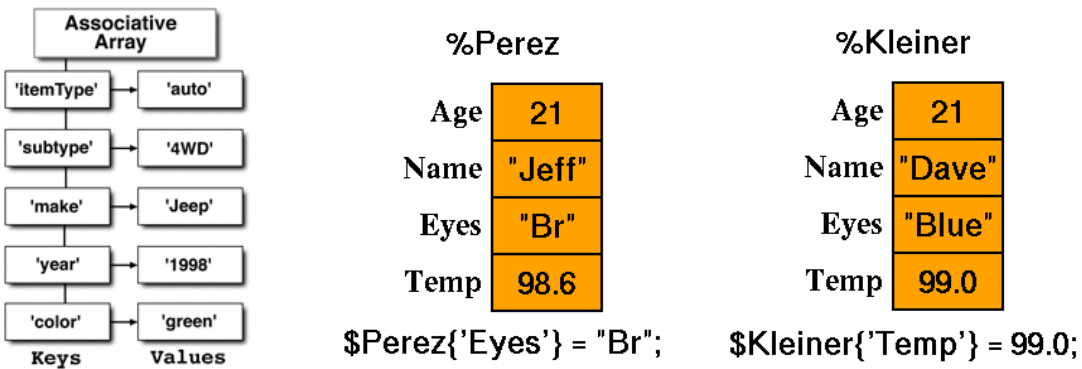
\includegraphics[width=0.43\textwidth]{c8_code_hash_01.png}}
      \item 简介:散列/关联数组\textcolor{red}{(和字典相类比)}
      \item 初始化:胖箭头(=>)
      \item 常见操作:keys,values,each,delete,exists
      \item 三种数据类型:标量变量 vs. 数组 vs. 散列
    \end{enumerate}
  \item 数据结构和算法(25分钟)\textcolor{red}{(通过基因表达的例子进行讲解)}
    \begin{enumerate}
      \item 简介:不同的算法通常需要不同的数据结构
      \item 排序:cmp(字符串),\verb|<=>|(数字),sort,折半查找
      \item 数据库:关系数据库(表格,行与列\textcolor{red}{(与Excel表格进行比较)}),SQL
      \item DBM:采用散列结构,与散列结合使用;dbmopen/dbmclose,tie/untie
    \end{enumerate}
  \item 遗传密码(25分钟)
    \begin{enumerate}
      \item 简介:密码子,三个核苷酸翻译成一个氨基酸
      \item \textcolor{red}{【重点】}策略:模式匹配,正则表达式,散列\textcolor{red}{(比较三种策略的优缺点)}
\parpic[fr]{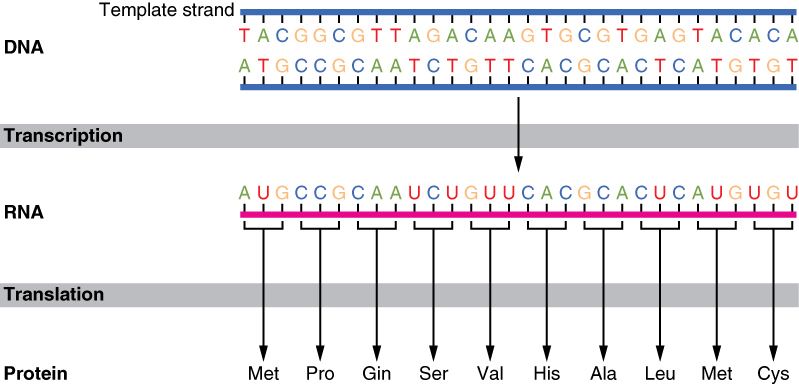
\includegraphics[width=0.4\textwidth]{c8_code_translation_01.jpg}}
      \item 知识点
	\begin{itemize}
	  \item 文件句柄:STDIN,STDOUT,STDERR
	  \item 正则表达式:元字符,选择,修饰符
	  \item 函数:uc(转换为大写),exists(检查键)
	\end{itemize}
    \end{enumerate}
  \item DNA翻译成蛋白质(20分钟)
    \begin{enumerate}
      \item Perl程序8.1:把DNA序列翻译成蛋白质序列
      \item \verb|for (my $i = 0; $i < (length($dna) - 2); $i += 3) {}|\textcolor{red}{(结合密码子的属性进行理解)}
      \item \verb|$codon = substr ($dna, $i, 3);|\textcolor{red}{(结合密码子的属性进行理解)}
      \item 把主程序变成子程序\textcolor{red}{(比较主程序和子程序的利弊)}
    \end{enumerate}
  \item 读取FASTA文件(60分钟)
    \begin{enumerate}
\parpic[fr]{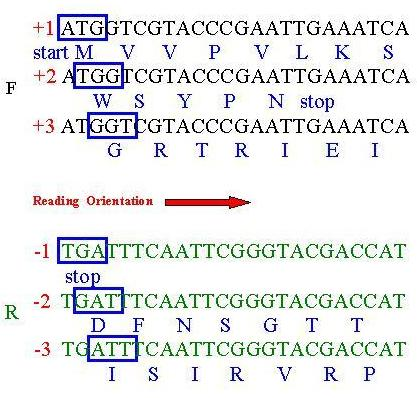
\includegraphics[width=0.38\textwidth]{c8_code_orf_01.jpg}}
      \item 序列格式:纯序列,FASTA,GenBank,EMBL,GCG,……
      \item 读取文件:一次性读入所有行,一次读入一行\textcolor{red}{(比较两种策略的优缺点)}
      \item 读取文件失败:退出程序,询问用户,使用默认文件,……\textcolor{red}{(比较各种方法的利弊)}
      \item Perl程序8.2:读取FASTA文件并从中提取序列数据\textcolor{red}{(体验子程序的优势)}
      \item Perl程序8.3:读取FASTA文件,把其中的序列翻译成蛋白质并进行格式化输出
    \end{enumerate}
  \item 阅读框(35分钟)
    \begin{enumerate}
      \item 简介:ORF,+1,+2,+3,-1,-2,-3
      \item 子程序库:充分利用已有的子程序,添加缺少的子程序
      \item Perl程序8.4:在六种框架下翻译DNA序列\textcolor{red}{(组合需要的子程序即可)}
      \item 索引方式:从0起始 vs.  从1起始\textcolor{red}{(注意面向程序和面向用户的选择)}
    \end{enumerate}

\otherTail
\newpage
\otherHeader

  \item 总结与答疑(5分钟)
    \begin{enumerate}
      \item 知识点
	\begin{itemize}
	  \item 散列:初始化,键值,常见操作及相关函数
	  \item 数据类型:标量变量,数组,散列
	  \item 正则表达式:元字符,字符集,修饰符,择一匹配
	  \item 其他:比较排序,文件句柄,循环,索引,……
	\end{itemize}
      \item 技能
	\begin{itemize}
	  \item 熟练使用Perl语言中的散列
	  \item 能编写把DNA翻译成蛋白质相关的Perl程序
	\end{itemize}
    \end{enumerate}
\end{enumerate}

\otherTail


\end{document}
